\section{\Large PROBLEM SET 3}
\subsection{PROBLEM 1}
\textit{Impose that satellite is axial-symmetric (Ix$=$Iy$\neq$Iz). Repeat numerical simulation from previous pset using initial condition 4) from previous pset.}

\begin{figure}[H]
\centering
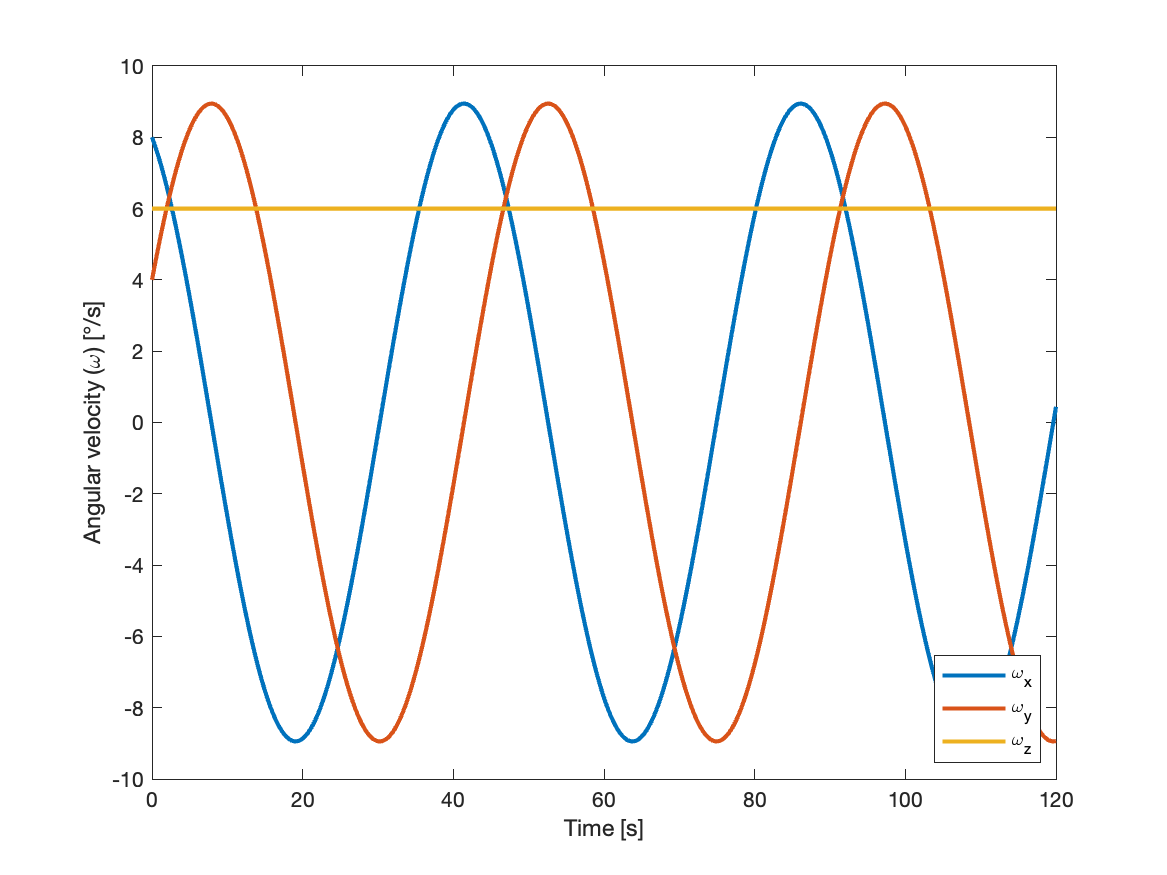
\includegraphics[scale=0.6]{Images/ps3_problem1.png}
\caption{Numerical solution results}
\label{fig:ps3_problem1}
\end{figure}


\subsection{PROBLEM 2}
\textit{Program analytical solution for axial-symmetric satellite. Compute it at same time steps and from same initial conditions.}

\begin{figure}[H]
\centering
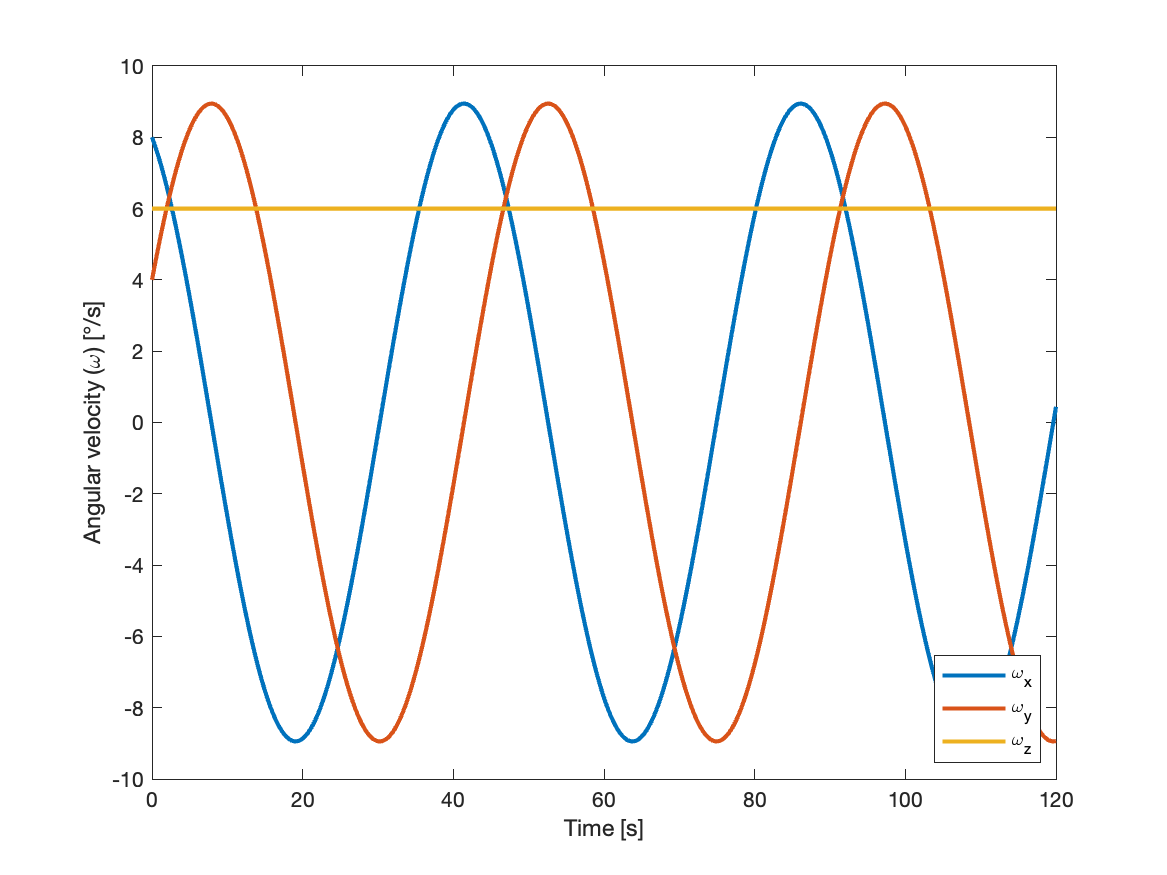
\includegraphics[scale=0.6]{Images/ps3_problem2.png}
\caption{Analytical solution results}
\label{fig:ps3_problem2}
\end{figure}


\subsection{PROBLEM 3}
\textit{Compare numerical and analytical solutions. Plot differences (errors), do not only superimpose absolute values. Tune numerical integrator for large discrepancies. Are angular velocity vector and angular momentum vector changing according to theory in principal axes?}

\begin{figure}[H]
\centering
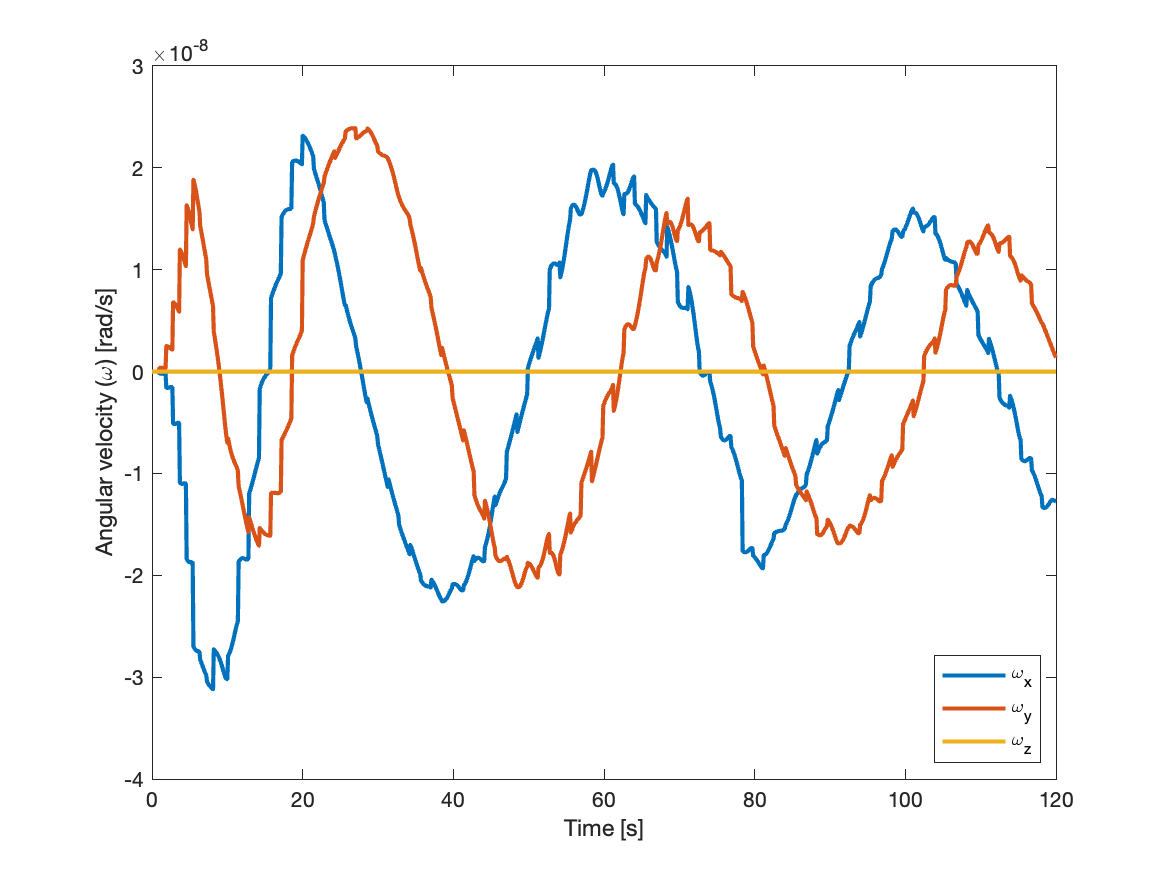
\includegraphics[scale=0.6]{Images/ps3_problem3.png}
\caption{Error between numerical and analytical solutions}
\label{fig:ps3_problem3}
\end{figure}


\subsection{PROBLEM 4}
\textit{Program Kinematic equations of motion correspondent to a nominal attitude parameterization of your choice.}

\lstinputlisting{src/kinQuaternion.m}

\lstinputlisting{src/kinQuaternionForwardEuler.m}

\lstinputlisting{src/kinQuaternionRK4.m}


\subsection{PROBLEM 5}
\textit{Program Kinematic equations of motion correspondent to a different attitude parameterization from the previous step. This is used for comparison, to get familiar with different approaches, and as fall back solution in the case of singularities.}

\lstinputlisting{src/kinEulerAngle.m}

\lstinputlisting{src/kinEulerAngleForwardEuler.m}


\subsection{PROBLEM 6}
\textit{Numerically integrate Euler AND Kinematic equations from arbitrary initial conditions (warning: stay far from singularity of adopted parameterization). Multiple revolutions. The output is the evolution of the attitude parameters over time. These attitude parameters describe orientation of principal axes relative to inertial axes.}


\subsection{PROBLEM 7}
\textit{ISince inertial position, velocity, and attitude, are known at the same time throughout the simulation, it is now possible to express vectors in the reference systems of interest.}

